\documentclass[conference,onecolumn]{IEEEtran}
\usepackage{enumitem}
%\usepackage{cite}
\usepackage{graphicx}
\usepackage{float}
\usepackage{amsmath, nccmath, bm}
\usepackage{amssymb}
\graphicspath{{./images}}
\usepackage[backend=biber,style=numeric]{biblatex}
\addbibresource{sources.bib}


\begin{document}
\section{Time Interleaver}
\subsection{Time Interleaver Overview}
XM requires time diversity in it's service to ensure a minimum dropout for paying customers.  To accomplish this, XM uses a convolutional time interleaver to spread the transmitted bits over a wide time (specifically 4.69 seconds).  Time diversity allows the receiver to recover the transmitted signal with large signal blockage time. 

\subsection{Time Interleaver XM}
In the XM radio MFP structure, the data is partitioned into PRC ``prime rate channels'' which consist of 258 PRC's grouped as 5440 transmitted bits each as seen in Figure {same as MFP/FSP figure}.  These 5440 bits PRS are the results of the FEC encoding which uses a RS(255,223) block code (Reed Solomon) followed by a convolutional encoding at rate 3/8.  A RS (255,223) encoder produces 2040 transmitted bits and the rate 3/8 convolution encoding increases the transmitted bits to 5440.  Each satellite transmits 1/2 the bits or 2720 bits.  Details of the FEC encoding will follow in FEC section.\\
Each PRC of 5440 bits per satellite is the result of 2 RS codewords.  As can be seen in Figure \ref{fig::time_interleaver} obtained from {CITE XM PATENT}, XM uses a separate convolutional time interleaver on each PRC \\

\begin{figure}[H]
	\centerline{\fbox{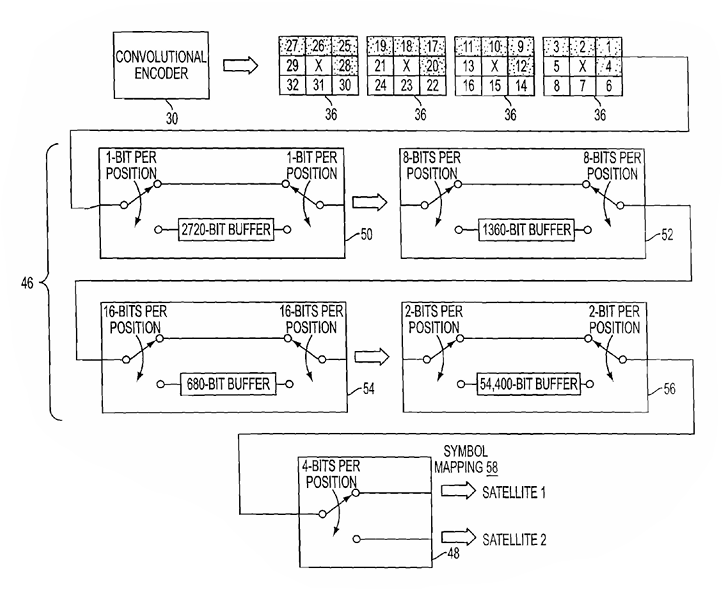
\includegraphics[width=0.8\textwidth]{XM_TIME_INTERLEAVER_DETAILS_no_label.png}}}
	\caption{XM Time Interleaver}
	\label{fig::time_interleaver}
\end{figure}
Figure \ref{fig::time_interleaver} shows the time interleaver from the transmission point of view.  The receiver follows in reverse. As can be seen each satellite can be processed independently or combined in a receiver through this time interleaver mechanism.  For the test, we used a single satellite (sat2) as the source and inserted zeros for the other satellite (sat1). Highlighted in block 36 is the punctured bits maked by an X and satellite 1 bits 1-4 and satellite 2 bits 5-8.  As can be seen in Figure \ref{fig::time_interleaver}, when one uses 5440 bits per MFP (.432mS) and calcuates the maximum delay through the 4 buffers, the result is an interleaver delay of 4.698s described in the XM chipset STA400a section 1.4 TDM DECODING {CITE}.

\section{Convolutional Decoder}
\subsection{Convolutional Decoder Overview}
A convolutional encoder/decoder uses a concept similar to FIR/IIR filters where the information bits are spead over time using GF(2).  These codes have been around since the 1950's.  These codes use registers to keep track of the state of the system.  They can be both recursive and non-recursive feedback polynomials to spread the information bits across time.  Non-recursive convolutional codes are commonly decoded with the Viterbi algorithm and recursive polynomials are commonly used in Turbo codes.

\subsection{Convolutional Decoder XM}
XM uses a non-recursive convolutional encoder/decoder as part of the concatenated coding.  Concatenated codes typically use an inner convolutional code with an outer block code.  For the XM sytem, they employ a complementary convolutional encoder.  This is a way to split the transmitted information across the two satellites as well as the terrestrial signal.  Figure \ref{fig::Viterbi} shows details of the convolution encoder described in XM patent {cite}.  This encoder takes in 3 information bits and create 9 transmitted bits.  The bits labeled ``A'', ``B'', ``C'' and ``D'' are sent to satellite 1 and bits ``F'', ``G'', ``H'' and ``J'' are sent to satellite 2.  The terrestrial signal uses the same bits as satellite 2 with the addition of bit ``E''.\\

Combining Figure \ref{fig::time_interleaver} and Figure \ref{fig::Viterbi} describe the convolutional encoding, bit puncturing and time interleaving of the XM system.
\begin{figure}[H]
	\centerline{\fbox{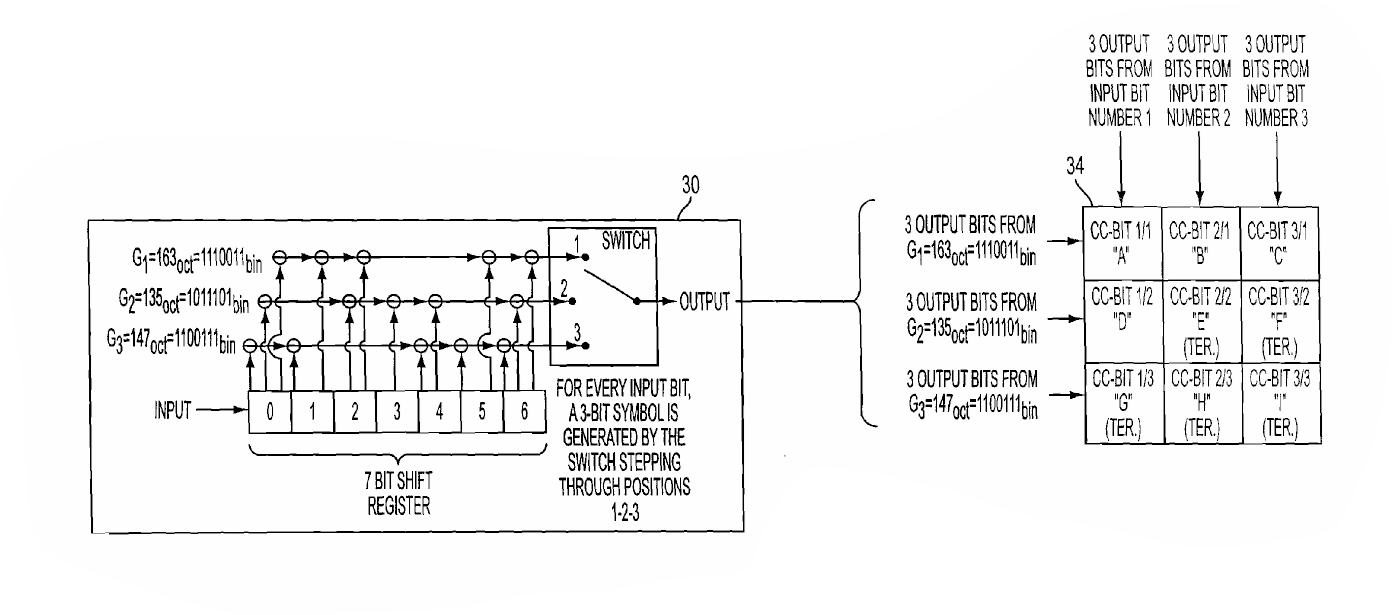
\includegraphics[width=0.8\textwidth]{Viterbi_encoder.png}}}
	\caption{XM Convolutional Encoder}
	\label{fig::Viterbi}
\end{figure}
\subsection{Procedure}  Taking the MFP aligned blocks, the first PRC (5440 bits) of satellite 2 was extracted following the description of the time interleaver.  These are mentioned at the TSCC (time slot control channel) and should contain a frame counter.  This was chosen as the best PRC to use as the channel structure is not expected to change constantly through a shorter time frame.  Because we were examining a single satellite, the time interleaver output to several frames to have enough transmitted bits to test against a Matlab Viterbi decoder.  With a single satellite, one can use either the top portion of the Viterbi decoder or the bottom portion depending on the chosen satellite.  With both satellites, one would chose to run the Viterbi as a rate 1/3 code rate.  With a single satellite one can use a rate 1/2 Viterbi with correct puncturing.  For a single satellite, the effective convolutional encoder rate is 3/4.  I.e. for every 4 received bits, there will be 3 usable information bits.  The decoder needs more than 3 transmission bits in order to determine the state of the trellis.

\begin{figure}[H]
	\centerline{\fbox{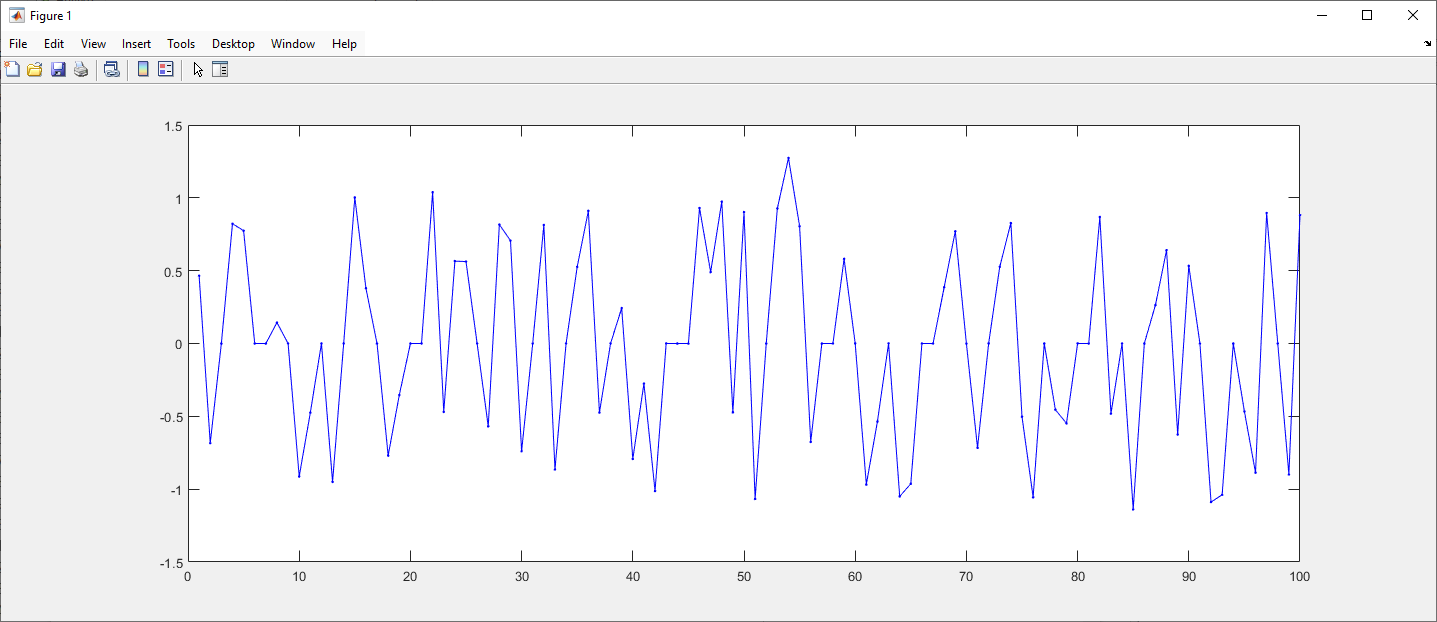
\includegraphics[width=0.8\textwidth]{Viterbi_insufficient_bits.png}}}
	\caption{XM Insufficient Data into Decoder}
	\label{fig::Viterbi_1}
\end{figure}
\begin{figure}[H]
	\centerline{\fbox{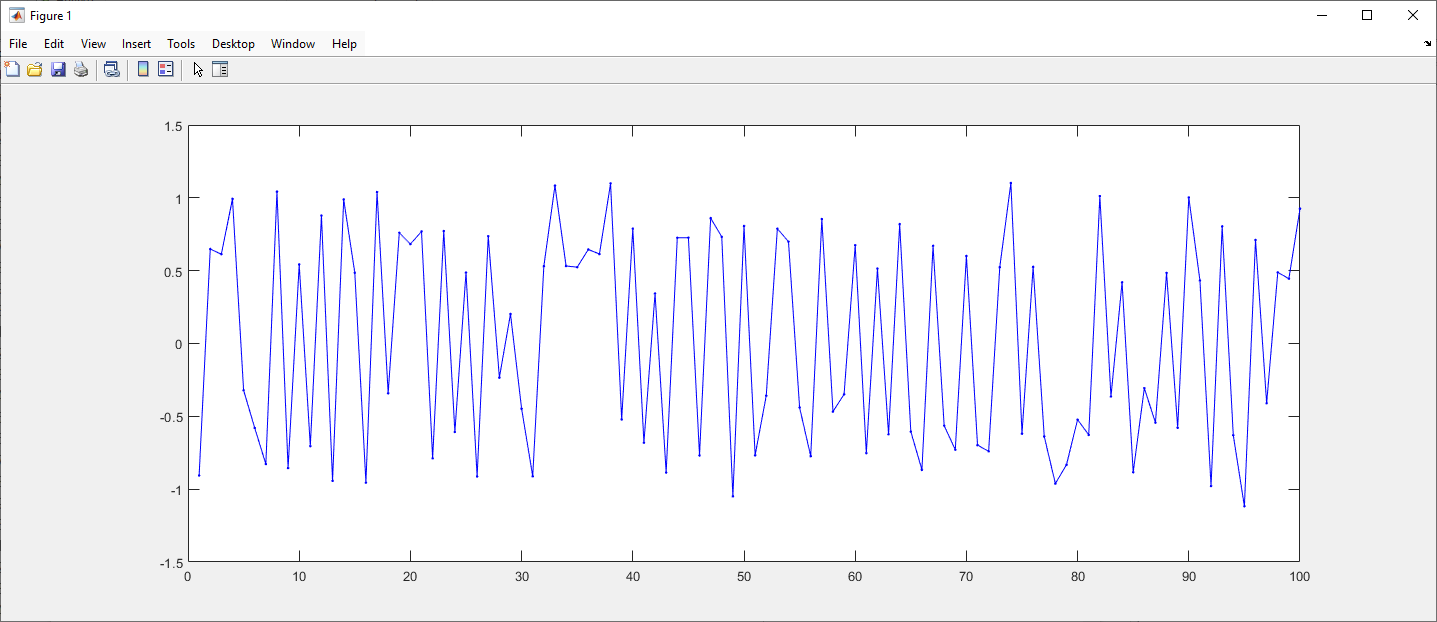
\includegraphics[width=0.8\textwidth]{Viterbi_sufficient_bits.png}}}
	\caption{XM Sufficient Data into Decoder}
	\label{fig::Viterbi_2}
\end{figure}

In Figure \ref{fig::Viterbi_1}, there is an insuffient number of input bits to a Viterbi decoder as the time interleaver is not completely full.  Since we are only using 1 satellite, the FEC is not capable of decoding this PRC block.  In Figure \ref{fig::Viterbi_2}, which is later in time, there is sufficient transmitted bits to use in the Viterbi decoder.\\

Next we looked at the Viterbi output for satellite 2.  This was done using the Matlab SPY plot.  As can be seen in Figure \ref{fig::Viterbi_spy}, the output does not show any structure in the vertical domain.  A frame counter was expected and not found.  
\begin{figure}[H]
	\centerline{\fbox{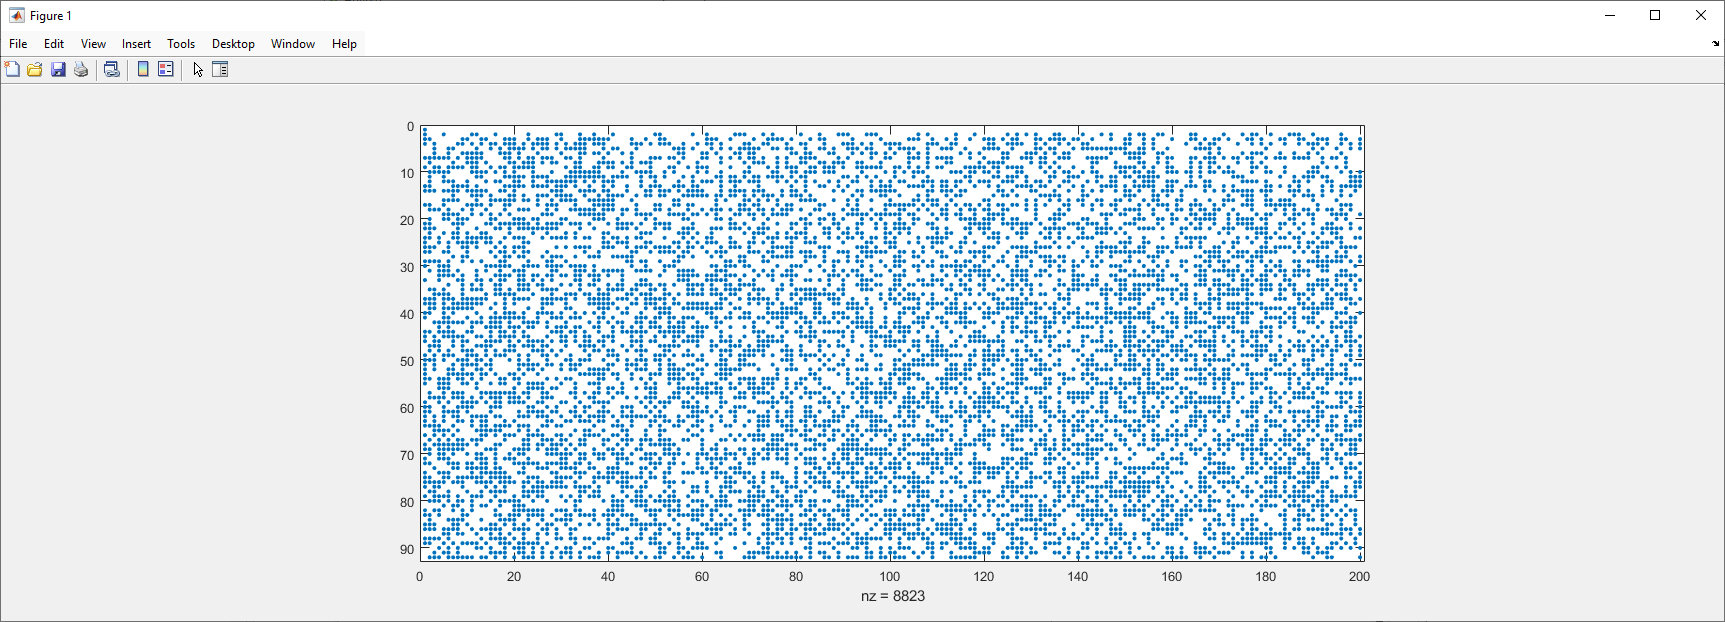
\includegraphics[width=0.8\textwidth]{Viterbi_SPY.png}}}
	\caption{XM Viterbi SPY output}
	\label{fig::Viterbi_spy}
\end{figure}
At this point we re-examined the documentation and discovered that the STA400a chipset showed a potential scrambler.  This was not included in any patent descriptions, not any mention in the STA400a document of the scrambler implementation.  So solve this unknown was outside the scope of the project.

\begin{figure}[H]
	\centerline{\fbox{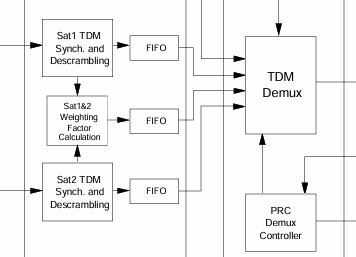
\includegraphics[width=0.8\textwidth]{XM_scrambler.png}}}
	\caption{XM potential scrambler}
	\label{fig::scrambler}
\end{figure}


\end{document}
